\documentclass{ximera}  


%\usepackage{todonotes}
%\usepackage{mathtools} %% Required for wide table Curl and Greens
%\usepackage{cuted} %% Required for wide table Curl and Greens
\newcommand{\todo}{}

\usepackage{esint} % for \oiint
\ifxake%%https://math.meta.stackexchange.com/questions/9973/how-do-you-render-a-closed-surface-double-integral
\renewcommand{\oiint}{{\large\bigcirc}\kern-1.56em\iint}
\fi


\graphicspath{
  {./}
  {jpg}
  {ximeraTutorial/}
  {basicPhilosophy/}
  {functionsOfSeveralVariables/}
  {normalVectors/}
  {lagrangeMultipliers/}
  {vectorFields/}
  {greensTheorem/}
  {shapeOfThingsToCome/}
  {dotProducts/}
  {partialDerivativesAndTheGradientVector/}
  {../productAndQuotientRules/exercises/}
  {../motionAndPathsInSpace/exercises/}
  {../normalVectors/exercisesParametricPlots/}
  {../continuityOfFunctionsOfSeveralVariables/exercises/}
  {../partialDerivativesAndTheGradientVector/exercises/}
  {../directionalDerivativeAndChainRule/exercises/}
  {../commonCoordinates/exercisesCylindricalCoordinates/}
  {../commonCoordinates/exercisesSphericalCoordinates/}
  {../greensTheorem/exercisesCurlAndLineIntegrals/}
  {../greensTheorem/exercisesDivergenceAndLineIntegrals/}
  {../shapeOfThingsToCome/exercisesDivergenceTheorem/}
  {../greensTheorem/}
  {../shapeOfThingsToCome/}
  {../separableDifferentialEquations/exercises/}
  {vectorFields/}
}

\newcommand{\mooculus}{\textsf{\textbf{MOOC}\textnormal{\textsf{ULUS}}}}

\usepackage{tkz-euclide}\usepackage{tikz}
\usepackage{tikz-cd}
\usetikzlibrary{arrows}
\tikzset{>=stealth,commutative diagrams/.cd,
  arrow style=tikz,diagrams={>=stealth}} %% cool arrow head
\tikzset{shorten <>/.style={ shorten >=#1, shorten <=#1 } } %% allows shorter vectors

\usetikzlibrary{backgrounds} %% for boxes around graphs
\usetikzlibrary{shapes,positioning}  %% Clouds and stars
\usetikzlibrary{matrix} %% for matrix
\usepgfplotslibrary{polar} %% for polar plots
\usepgfplotslibrary{fillbetween} %% to shade area between curves in TikZ
\usetkzobj{all}
\usepackage[makeroom]{cancel} %% for strike outs
%\usepackage{mathtools} %% for pretty underbrace % Breaks Ximera
%\usepackage{multicol}
\usepackage{pgffor} %% required for integral for loops



%% http://tex.stackexchange.com/questions/66490/drawing-a-tikz-arc-specifying-the-center
%% Draws beach ball
\tikzset{pics/carc/.style args={#1:#2:#3}{code={\draw[pic actions] (#1:#3) arc(#1:#2:#3);}}}



\usepackage{array}
\setlength{\extrarowheight}{+.1cm}
\newdimen\digitwidth
\settowidth\digitwidth{9}
\def\divrule#1#2{
\noalign{\moveright#1\digitwidth
\vbox{\hrule width#2\digitwidth}}}





\newcommand{\RR}{\mathbb R}
\newcommand{\R}{\mathbb R}
\newcommand{\N}{\mathbb N}
\newcommand{\Z}{\mathbb Z}

\newcommand{\sagemath}{\textsf{SageMath}}


%\renewcommand{\d}{\,d\!}
\renewcommand{\d}{\mathop{}\!d}
\newcommand{\dd}[2][]{\frac{\d #1}{\d #2}}
\newcommand{\pp}[2][]{\frac{\partial #1}{\partial #2}}
\renewcommand{\l}{\ell}
\newcommand{\ddx}{\frac{d}{\d x}}

\newcommand{\zeroOverZero}{\ensuremath{\boldsymbol{\tfrac{0}{0}}}}
\newcommand{\inftyOverInfty}{\ensuremath{\boldsymbol{\tfrac{\infty}{\infty}}}}
\newcommand{\zeroOverInfty}{\ensuremath{\boldsymbol{\tfrac{0}{\infty}}}}
\newcommand{\zeroTimesInfty}{\ensuremath{\small\boldsymbol{0\cdot \infty}}}
\newcommand{\inftyMinusInfty}{\ensuremath{\small\boldsymbol{\infty - \infty}}}
\newcommand{\oneToInfty}{\ensuremath{\boldsymbol{1^\infty}}}
\newcommand{\zeroToZero}{\ensuremath{\boldsymbol{0^0}}}
\newcommand{\inftyToZero}{\ensuremath{\boldsymbol{\infty^0}}}



\newcommand{\numOverZero}{\ensuremath{\boldsymbol{\tfrac{\#}{0}}}}
\newcommand{\dfn}{\textbf}
%\newcommand{\unit}{\,\mathrm}
\newcommand{\unit}{\mathop{}\!\mathrm}
\newcommand{\eval}[1]{\bigg[ #1 \bigg]}
\newcommand{\seq}[1]{\left( #1 \right)}
\renewcommand{\epsilon}{\varepsilon}
\renewcommand{\phi}{\varphi}


\renewcommand{\iff}{\Leftrightarrow}

\DeclareMathOperator{\arccot}{arccot}
\DeclareMathOperator{\arcsec}{arcsec}
\DeclareMathOperator{\arccsc}{arccsc}
\DeclareMathOperator{\si}{Si}
\DeclareMathOperator{\scal}{scal}
\DeclareMathOperator{\sign}{sign}


%% \newcommand{\tightoverset}[2]{% for arrow vec
%%   \mathop{#2}\limits^{\vbox to -.5ex{\kern-0.75ex\hbox{$#1$}\vss}}}
\newcommand{\arrowvec}[1]{{\overset{\rightharpoonup}{#1}}}
%\renewcommand{\vec}[1]{\arrowvec{\mathbf{#1}}}
\renewcommand{\vec}[1]{{\overset{\boldsymbol{\rightharpoonup}}{\mathbf{#1}}}\hspace{0in}}

\newcommand{\point}[1]{\left(#1\right)} %this allows \vector{ to be changed to \vector{ with a quick find and replace
\newcommand{\pt}[1]{\mathbf{#1}} %this allows \vec{ to be changed to \vec{ with a quick find and replace
\newcommand{\Lim}[2]{\lim_{\point{#1} \to \point{#2}}} %Bart, I changed this to point since I want to use it.  It runs through both of the exercise and exerciseE files in limits section, which is why it was in each document to start with.

\DeclareMathOperator{\proj}{\mathbf{proj}}
\newcommand{\veci}{{\boldsymbol{\hat{\imath}}}}
\newcommand{\vecj}{{\boldsymbol{\hat{\jmath}}}}
\newcommand{\veck}{{\boldsymbol{\hat{k}}}}
\newcommand{\vecl}{\vec{\boldsymbol{\l}}}
\newcommand{\uvec}[1]{\mathbf{\hat{#1}}}
\newcommand{\utan}{\mathbf{\hat{t}}}
\newcommand{\unormal}{\mathbf{\hat{n}}}
\newcommand{\ubinormal}{\mathbf{\hat{b}}}

\newcommand{\dotp}{\bullet}
\newcommand{\cross}{\boldsymbol\times}
\newcommand{\grad}{\boldsymbol\nabla}
\newcommand{\divergence}{\grad\dotp}
\newcommand{\curl}{\grad\cross}
%\DeclareMathOperator{\divergence}{divergence}
%\DeclareMathOperator{\curl}[1]{\grad\cross #1}
\newcommand{\lto}{\mathop{\longrightarrow\,}\limits}

\renewcommand{\bar}{\overline}

\colorlet{textColor}{black}
\colorlet{background}{white}
\colorlet{penColor}{blue!50!black} % Color of a curve in a plot
\colorlet{penColor2}{red!50!black}% Color of a curve in a plot
\colorlet{penColor3}{red!50!blue} % Color of a curve in a plot
\colorlet{penColor4}{green!50!black} % Color of a curve in a plot
\colorlet{penColor5}{orange!80!black} % Color of a curve in a plot
\colorlet{penColor6}{yellow!70!black} % Color of a curve in a plot
\colorlet{fill1}{penColor!20} % Color of fill in a plot
\colorlet{fill2}{penColor2!20} % Color of fill in a plot
\colorlet{fillp}{fill1} % Color of positive area
\colorlet{filln}{penColor2!20} % Color of negative area
\colorlet{fill3}{penColor3!20} % Fill
\colorlet{fill4}{penColor4!20} % Fill
\colorlet{fill5}{penColor5!20} % Fill
\colorlet{gridColor}{gray!50} % Color of grid in a plot

\newcommand{\surfaceColor}{violet}
\newcommand{\surfaceColorTwo}{redyellow}
\newcommand{\sliceColor}{greenyellow}




\pgfmathdeclarefunction{gauss}{2}{% gives gaussian
  \pgfmathparse{1/(#2*sqrt(2*pi))*exp(-((x-#1)^2)/(2*#2^2))}%
}


%%%%%%%%%%%%%
%% Vectors
%%%%%%%%%%%%%

%% Simple horiz vectors
\renewcommand{\vector}[1]{\left\langle #1\right\rangle}


%% %% Complex Horiz Vectors with angle brackets
%% \makeatletter
%% \renewcommand{\vector}[2][ , ]{\left\langle%
%%   \def\nextitem{\def\nextitem{#1}}%
%%   \@for \el:=#2\do{\nextitem\el}\right\rangle%
%% }
%% \makeatother

%% %% Vertical Vectors
%% \def\vector#1{\begin{bmatrix}\vecListA#1,,\end{bmatrix}}
%% \def\vecListA#1,{\if,#1,\else #1\cr \expandafter \vecListA \fi}

%%%%%%%%%%%%%
%% End of vectors
%%%%%%%%%%%%%

%\newcommand{\fullwidth}{}
%\newcommand{\normalwidth}{}



%% makes a snazzy t-chart for evaluating functions
%\newenvironment{tchart}{\rowcolors{2}{}{background!90!textColor}\array}{\endarray}

%%This is to help with formatting on future title pages.
\newenvironment{sectionOutcomes}{}{}



%% Flowchart stuff
%\tikzstyle{startstop} = [rectangle, rounded corners, minimum width=3cm, minimum height=1cm,text centered, draw=black]
%\tikzstyle{question} = [rectangle, minimum width=3cm, minimum height=1cm, text centered, draw=black]
%\tikzstyle{decision} = [trapezium, trapezium left angle=70, trapezium right angle=110, minimum width=3cm, minimum height=1cm, text centered, draw=black]
%\tikzstyle{question} = [rectangle, rounded corners, minimum width=3cm, minimum height=1cm,text centered, draw=black]
%\tikzstyle{process} = [rectangle, minimum width=3cm, minimum height=1cm, text centered, draw=black]
%\tikzstyle{decision} = [trapezium, trapezium left angle=70, trapezium right angle=110, minimum width=3cm, minimum height=1cm, text centered, draw=black]




 
\title{Review of Phasors} 
\author{Milica Markovic} 
\outcome{Apply phasor transformation to a time-domain equation to obtain frequency-domain equation.}
\begin{document}  
\begin{abstract}  
Phasors are essential tool in circuit analysis.
\end{abstract}  
\maketitle    


\begin{definition}
Phasor transformation is defined as follows:

\begin{eqnarray}
v(t)=\Re\{|V|e^{j\theta_v} e^{j \omega t}\}
\end{eqnarray}

where $|\widetilde{V}|e^{j\theta_v}$ is the phasor of voltage $v(t)$. Phasor is a complex number in polar coordinate system and it is usually denoted with a capital letter with a tilde above it $\widetilde{V} = |\widetilde{V}|e^{j\theta_v}$. $ |\widetilde{V}|$ is the magnitude and $\theta_v$ is the phase of the complex number. Symbol $\Re$ represents the real part of the expression in the curly brackets. 

\end{definition}

You may be wondering why would this specific equation be used. This is the case of inverse superposition. We add an addition voltage source to our circuit, denote it as imaginary by multiplying it with $j=\sqrt{-1}$, so that we are able to use the Eurler's formula to write a sinusoidal signals in terms of complex exponentials. When we use complex exponentials, the time-domain differential equations transform to simple algebraic equations. Principle of superpositions tells us that the response of the circuit to the real part of the generator will be real, and the response of the imaginary part of the generator will be imaginary. Since we added additional source that wasn't there previously, we now need to take the response only from the real generator.

\begin{example}

We will see how is the phasor transformation applied to an RC circuit shown in Figure \ref{RCcirc}.  To solve this circuit in the time domain we apply Kirchoff's voltage law as shown in Equation \ref{eq-1} -\ref{eq0}.


The circuit in Figure \ref{RCcirc} is a simple RC circuit. KVL equation in the time domain is given in Equation \ref{eq-1}.

\begin{eqnarray}
        v_s(t)=v_R(t)+v_C(t)                \label{eq-1}  \\
v_s(t) = R i + \frac{1}{C} \int i(t) dt \label{eq0}
\end{eqnarray} 


\begin{figure}[htbp]
\begin{center}
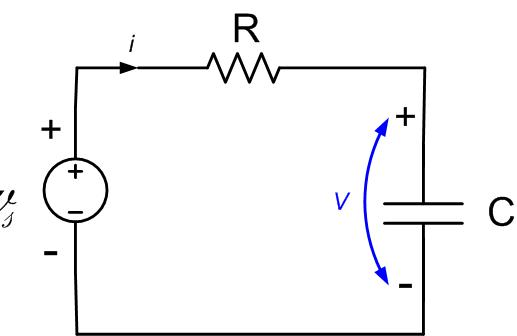
\includegraphics[scale=0.3]{../jpg/RCnew.jpg}
%\strut\psfig{figure=complexnumberz.ps,width=3cm} \\
\end{center}
\caption{Complex number z in rectangular and polar coordinates.}
\label{RCcirc}
\end{figure}




Where
\begin{eqnarray}
v_s(t)= A cos (\omega t + \Theta ) \label{eq1}
\end{eqnarray}

In order to solve this circuit we have to  solve a differential equation.
Use of phasors simplify the equations
significantly. Differential equations become a set of
linear equations.  Phasor is another name for a complex number  in polar coordinate system. 

In order to use phasors, the circuit has to be linear. Circuits that have  only capacitors, inductors and resistors are 
linear circuits.  In  a  linear circuit, all currents and voltages are  at the frequency of the generator. That means that we don't have to keep track  of the frequency of voltages and currents when we are solving the circuit. We know the frequency once we know the frequency of the generator. The quantities that will differ for different currents and voltages  is the amplitude and phase of the signal. Phasors allow us to drop the information about the frequency of the signal, and only  keep track of the magnitude and phase of the signal.
 In order to remove $cos (\omega t)$  term from the equations 
we have to use complex numbers.  To write $cos (\omega t)$ \footnote{It is customary to use  $\cos( \omega t)$ for our time-domain signal. If signals in a circuit are given in terms of $\sin (\omega t)$, the sin function has to be converted to a cosine. To do that, subtract $90^o$ from the phase of the sinusoid, because $\sin( \omega t) = \cos(\omega t - 90^o)$}  in a concise form  as a complex number, we add to the forcing function  a sinusoidal imaginary term.

\begin{eqnarray}
 A \cos (\omega t + \Theta ) + j A sin (\omega t + \Theta)
\end{eqnarray}

We have to make sure later  when we are done with our calculations with complex number, that we only take the real part of the final expression. It seems that we made the above expression more complicated,  however, if we
remember Euler's identity, the expression becomes


\begin{eqnarray}
v_s(t)=  V \cos (\omega t + \Theta_V)=\Re\{ A cos (\omega t + \Theta ) + j A sin (\omega t + \Theta)\}= \nonumber \\ 
= \Re\{A e^{j(\omega t + \Theta)}\}=\Re\{A e^{j \Theta} e^{j \omega t}\} \label{eq2}
\end{eqnarray}

In Equation \ref{eq2}  we  extracted the phase and amplitude information
and separated it from the frequency. The amplitude and phase information is called phasor $V_S (j \omega)=A e^{j \Theta}$. 
Why is this expression better then the one with a $cos(\omega t)$ and how can we remove t from  Equation \ref{eq0}? To answer this question, we first have to write general expressions for voltage $v(t)$ and current $ i(t)$ in the Equation \ref{eq0}:

\begin{eqnarray}
v(t)= \Re\{ V cos (\omega t + \Theta_V ) + j V \sin (\omega t + \Theta_V)\}= \nonumber \\ =\Re\{V e^{j(\omega t + \Theta_V)}\}=\Re\{V e^{j \Theta_V} e^{j \omega t}\} \label{eq41}
\end{eqnarray}

If we look at the first and last expression in Equation \ref{eq41} we see that the time domain signal is  the real part of the product of phasor and  the $e^{j \omega t}$ term. 

\begin{eqnarray}
v(t)=\Re\{V e^{j \Theta_V} e^{j \omega t}\} \label{eq41a} 
\end{eqnarray}

Similarly for current

\begin{eqnarray}
i(t)= I \cos (\omega t + \Theta_I) =\Re\{ I cos (\omega t + \Theta_I) + j I \sin (\omega t + \Theta_I)\}= \nonumber \\ =\Re\{I e^{j(\omega t + \Theta_I)}\}=\Re\{I e^{j \Theta_I} e^{j \omega t}\} \label{eq51} 
\end{eqnarray}




If we look at the first and last expression in Equation \ref{eq51} we get a similar expression for current.

\begin{eqnarray}
i(t)= \Re\{I e^{j \Theta_I} e^{j \omega t}\} \label{eq51a}
\end{eqnarray}



 In Equations  \ref{eq41}-\ref{eq51}    $V$ and $I$ are voltage and current amplitudes, and $\Theta_V $ and $\Theta_I$  are voltage and current phases. The voltage on the resistor is then given in Equation \ref{voltres} 

\begin{eqnarray}
v_R(t)=R \times  i(t) =  R \times  Re\{I e^{j \Theta_I} e^{j \omega t}\}  =   \Re\{R \times I e^{j \Theta_I} e^{j \omega t}\}   \label{voltres}
\end{eqnarray}

The voltage on the capacitor is a bit more complicated. We know that $i(t)=\Re\{I e^{j \Theta_I} e^{j \omega t}\}$, but what is the integral of $i(t)$?



\begin{eqnarray}
v_C(t) =  \frac{1}{C} \int \Re\{I e^{j \Theta_I} e^{j \omega t}\}  dt \label{eq6}
\end{eqnarray} 

Now if integral and $Re$ exchange places, and if we take all time-independent quantities in front of the integral,



\begin{eqnarray}
v_C(t) = \frac{1}{C} \int i(t) dt  =  \Re\{   \frac{1}{C} \int I e^{j \Theta_I} e^{j \omega t}\}  dt  = \Re\{   \frac{1}{C}  I e^{j \Theta_I} \int e^{j \omega t}dt \}   \label{eq7} \\
v_C(t)= \Re\{   \frac{1}{C}  I e^{j \Theta_I} \frac{1}{j \omega} e^{j \omega t}  \}   = \Re\{   \frac{1}{j \omega C}  I e^{j \Theta_I}  e^{j \omega t}  \}  \label{eq8}
\end{eqnarray} 




%\begin{center}
%\begin{tabular}{|c|c|} \hline
%$ i(t)$ & $I(j \omega)   e^{j\omega t}$    \\  \hline       
%$ v(t)$ & $V(j \omega)   e^{j\omega t}$ \\ \hline
%$ \frac{v(t)}{dt}$ & $j \omega V(j \omega)   e^{j\omega t}$ \\ \hline
%$ \int  i(t) dt$ & $\frac{I(j \omega)}{j \omega}   e^{j\omega t}$ \\ \hline
%\end{tabular}
%\end{center}


We now replace the time-domain quantities in equation \ref{eq0} with
these newly developed expressions.



\begin{eqnarray}
v_s(t)=v_R(t) + v_C(t)  \\
Re\{A e^{j \Theta} e^{j \omega t}\}=    \Re\{R \times I e^{j \Theta_I} e^{j \omega t}\}   +  \Re\{   \frac{1}{j \omega C}  I e^{j \Theta_I}  e^{j \omega t}  \}
\end{eqnarray}

A common term in the previous equation is $ e^{j\omega t}$, and we can now drop $Re$, as long as we later remember to take only the real part of the expresion for the phasor of voltage and current to get the time domain expression. We can now
write the equation as




\begin{eqnarray}
 V_S  e^{j \Theta_{V_S}}  =R \times I e^{j \Theta_I}  +    \frac{1}{j \omega C}  I e^{j \Theta_I}  \\
V_S(j \omega)   = R I(j \omega)    + \frac{I(j \omega )}{j \omega C} 
\end{eqnarray}

\end{example}

Since this is a linear equation, we can easily solve it:


\begin{eqnarray}
I (j \omega) = \frac{V_S(j \omega)}{ R    + \frac{1}{j \omega C} } \label{pheq}
\end{eqnarray} 



Let's say that the values  are given for R, C,  $\omega$  and $V_S$ such that the phasor of the current is  $I=3 e^{j 45^o}$. To obtain the signal in the time domain,  we   multiply the phasor $I$ with the $ e^{j\omega t}$ term, and  then we find
the real part of the expression to obtain its current in the time domain, as shown in Figure \ref{phtotd}


\begin{eqnarray}
i(t) = \Re\{ 3 e^{j 45^o}  e^{j\omega t} \} =  Re\{3 e^{j \omega t + 45^o}  \} = \nonumber \\ = \Re \{ 3 \cos (\omega t + 45^o ) + j 3 \sin (\omega t + 45^o \} = 3  \cos (\omega t + 45^o ) \label{phtotd}
\end{eqnarray}

In case we have an inductor in the circuit, the voltage on an inductor can be derived as shown in Figure \ref{eq77}. 


\begin{eqnarray}
v_L(t) = L \frac{\partial{ i(t)}}{\partial t}  =L  \frac{ Re\{    I e^{j \Theta_I} e^{j \omega t}\}}{\partial t}  dt  = \Re\{  LI e^{j \Theta_I} \frac{ \partial e^{j \omega t}}{\partial t} \} =  \nonumber \\ = \Re\{  LI e^{j  \Theta_I}  j  \omega e^{j \omega t} \} =  \Re \{  j  \omega       LI e^{j  \Theta_I}    e^{j \omega t}   \}      \label{eq77} 
\end{eqnarray}


\begin{figure}[htbp]
\begin{center}
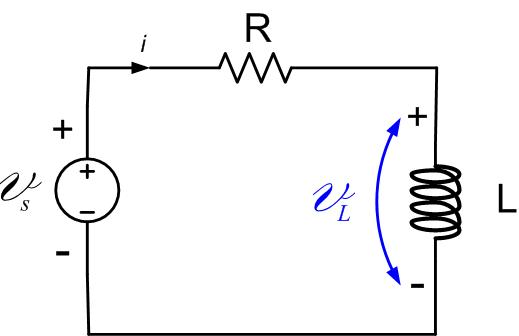
\includegraphics[scale=0.3]{../jpg/RLnew.jpg}
%\strut\psfig{figure=complexnumberz.ps,width=3cm} \\
\end{center}
\caption{Complex number z in rectangular and polar coordinates.}
\label{RLcirc}
\end{figure}



 Step-by-step instructions on how to solve circuits using phasors is given as follows:
\begin{enumerate}
\item Adopt cosine reference for generator voltage or current. 
\item replace all impedances with their phasor expressions,
\item write KVL and KCL, or use other Network Analysis techniques.
\item find the phasor expression for the required current or voltage. 
\item multiply the phasor with $e^{j \omega t}$  
\item find the real part of the above expression to get the current in the time domain.
\end{enumerate}






\begin{table}
\centering
\begin{tabular}{|c|c|c|c|c|} \hline
cicruit element & impedance & low frequencies $f \to 0$& high frequencies $f \to \inf$   \\  \hline  
 capacitor     & $\frac{1}{j \omega C}$    & $\infty$ & $0$    \\  \hline       
 inductor & $j \omega L$              &    $0$   &       $\infty $             \\ \hline
\end{tabular}
\caption{Impedance of the capacitor and inductors and their equivalent impedances at high and low frequencies.}
\end{table}



\begin{example}
Using Vectors to Represent Phasors in an example


 Calculate on paper the magnitude  and phase of the current and voltages in a series RC circuit shown in Figure \ref{f112} (a) if the circuit is driven with a frequency of 1\,GHz (phase is zero) and R=1k$\Omega $, C= ${\frac{1}{2\pi }10}^{-12}$F. 
 
 
 Answer the following questions:

\begin{enumerate}
\item  What are the magnitude, phase and time delay of the source voltage?

\item  What are the magnitude, phase and time delay of the voltage across the resistor?

\item  What are the magnitude, phase and time delay of the voltage across the capacitor?

\item  The simulated voltage magnitude across the resistor is about 0.5V and the simulated voltage across the capacitor is about 0.85V.  If we use KVL $ 0.85V+0.5V \neq 1V$. Why? Look at Figure \ref{f112} to help you with answer this question.

\end{enumerate}
\begin{explanation} 
 
 
  When you calculate the magnitudes and phases of the voltages in the RC circuit, draw three points, to represent magnitude and phases of all three vectors, as in Figure \ref{PP}. The three points denote the three position vectors as shown in Figure \ref{f112}. Vector addition must be used to add the voltages on the resistor and capacitor to obtain the voltage of the generator. 






\begin{figure}[htbp]
%\vspace*{-0.5cm}
\begin{center}
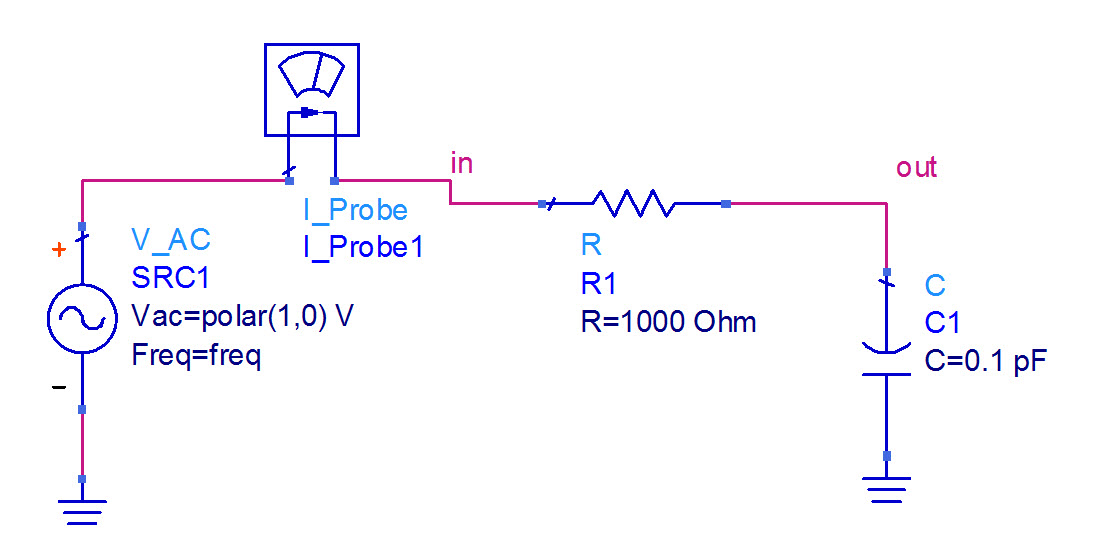
\includegraphics[scale=0.2]{../jpg/RCcircADS.jpg}
\end{center}
\caption{\label{RCcircADS} RC circuit in ADS.}
\end{figure}


\begin{figure}[htbp]
%\vspace*{-0.5cm}
\begin{center}
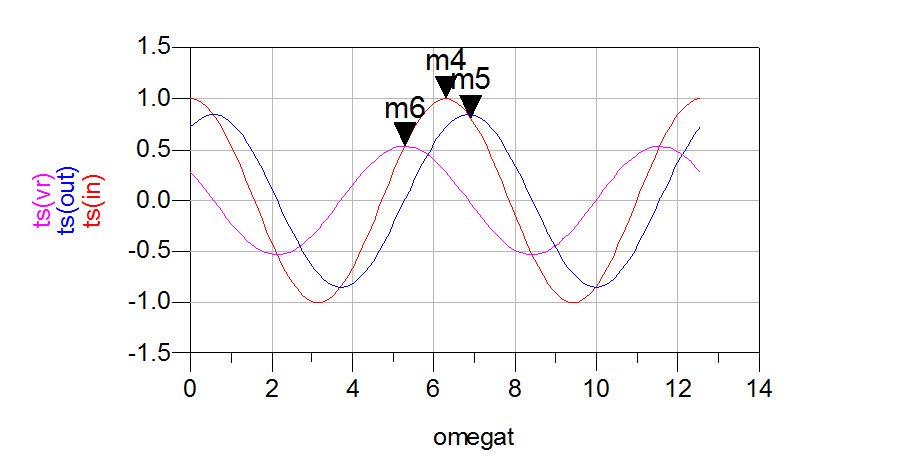
\includegraphics[scale=0.3]{../jpg/voltagesinRCcircRadADS}
\end{center}
\caption{\label{SSangle} Sinusoidal signal as a function of angle $\omega t$}
\end{figure}


\begin{figure}[htbp]
%\vspace*{-0.5cm}
\begin{center}
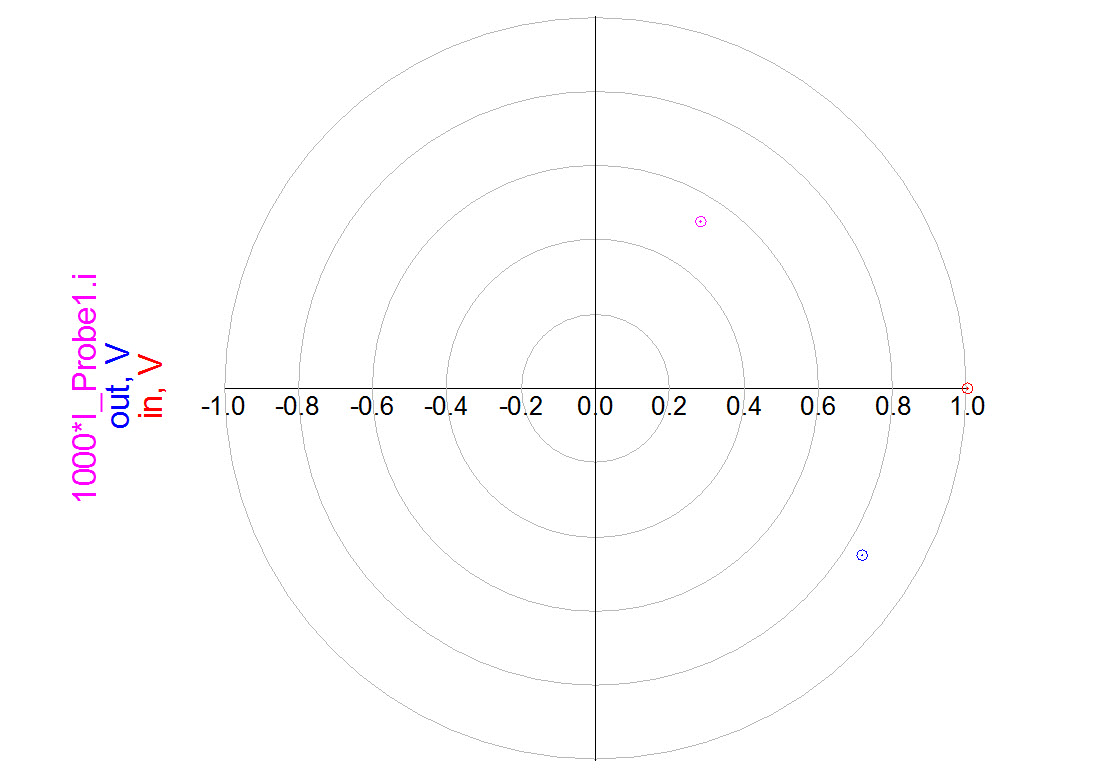
\includegraphics[scale=0.2]{../jpg/RCvoltPolarPlotADS.jpg}
\end{center}
\caption{\label{PP} Points represent polar plot of complex voltages in RC circuit.}
\end{figure}


\begin{figure}[htbp]
%\vspace*{-0.5cm}
\begin{center}
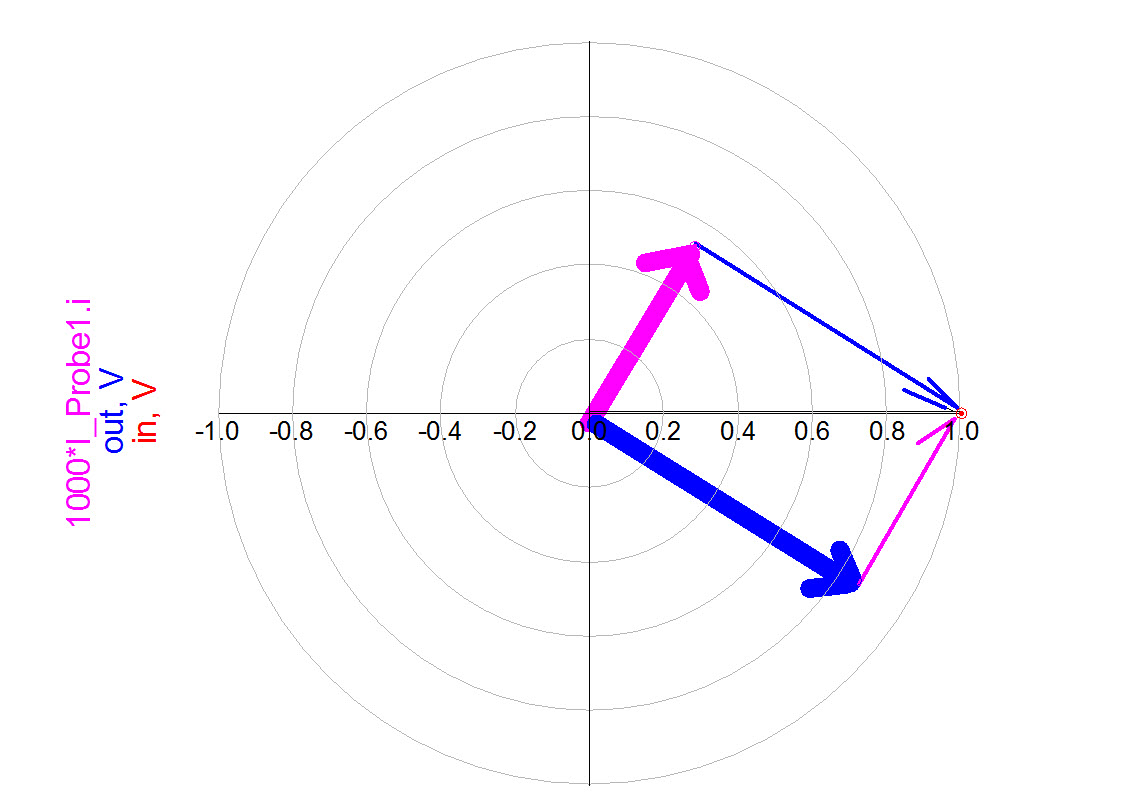
\includegraphics[scale=0.2]{../jpg/RCvoltPolarPlotVectors.jpg}
\end{center}
\caption{\label{f112} Vectors are drawn in the polar plot of complex voltages in RC circuit. Note how they add up to 1V.}
\end{figure}





%\begin{figure}[htbp]
%\vspace*{-0.5cm}
%\begin{center}
%\includegraphics[scale=0.7]{../jpg/addingvectors.jpg}
%\end{center}
%\caption{\label{f113} Skeching phasors using vector magnitudes on paper.}
%\end{figure}
\end{explanation}



\end{example}





%This activity is about creative work.  
%\begin{exercise}  
%  Choose the best place to work on mathematics.  
%  \begin{multipleChoice}  
%    \choice{At the library}  
%    \choice[correct]{At the caffe}  
%    \choice{In your office}  
%  \end{multipleChoice}  
%\end{exercise}  



\begin{sageCell}
var('s t')
x(t) = 3*cos(t)
y(t) = 3*sin(t)
c(t) = (x(t),y(t))
circle=parametric_plot(c(t),(t,0,2*pi),color="black")
circle
\end{sageCell}

\begin{sageOutput}
var('s t')
x(t) = 3*cos(t)
y(t) = 3*sin(t)
c(t) = (x(t),y(t))
circle=parametric_plot(c(t),(t,0,2*pi),color="black")
circle
\end{sageOutput}

\end{document} 
